\documentclass[letterpaper]{article}
\usepackage[margin=1in]{geometry}
\usepackage[utf8]{inputenc}
\usepackage{textcomp}
\usepackage{amssymb}
\usepackage{natbib}
\usepackage{graphicx}
\usepackage{gensymb}
\usepackage{amsthm, amsmath, mathtools}
\usepackage[dvipsnames]{xcolor}
\usepackage{enumerate}
\usepackage{mdframed}
\usepackage[most]{tcolorbox}
\usepackage{csquotes}
% https://tex.stackexchange.com/questions/13506/how-to-continue-the-framed-text-box-on-multiple-pages

\tcbuselibrary{theorems}

\newcommand{\R}{\mathbb{R}}
\newcommand{\Z}{\mathbb{Z}}
\newcommand{\N}{\mathbb{N}}
\newcommand{\Q}{\mathbb{Q}}
\newcommand{\C}{\mathbb{C}}
\newcommand{\code}[1]{\texttt{#1}}
\newcommand{\mdiamond}{$\diamondsuit$}
\newcommand{\PowerSet}{\mathcal{P}}
\newcommand{\Mod}[1]{\ (\mathrm{mod}\ #1)}
\DeclareMathOperator{\lcm}{lcm}

%\newtheorem*{theorem}{Theorem}
%\newtheorem*{definition}{Definition}
%\newtheorem*{corollary}{Corollary}
%\newtheorem*{lemma}{Lemma}
\newtheorem*{proposition}{Proposition}


\newtcbtheorem[number within=section]{theorem}{Theorem}
{colback=green!5,colframe=green!35!black,fonttitle=\bfseries}{th}

\newtcbtheorem[number within=section]{definition}{Definition}
{colback=blue!5,colframe=blue!35!black,fonttitle=\bfseries}{def}

\newtcbtheorem[number within=section]{corollary}{Corollary}
{colback=yellow!5,colframe=yellow!35!black,fonttitle=\bfseries}{cor}

\newtcbtheorem[number within=section]{lemma}{Lemma}
{colback=red!5,colframe=red!35!black,fonttitle=\bfseries}{lem}

\newtcbtheorem[number within=section]{example}{Example}
{colback=white!5,colframe=white!35!black,fonttitle=\bfseries}{def}

\newtcbtheorem[number within=section]{note}{Important Note}{
        enhanced,
        sharp corners,
        attach boxed title to top left={
            xshift=-1mm,
            yshift=-5mm,
            yshifttext=-1mm
        },
        top=1.5em,
        colback=white,
        colframe=black,
        fonttitle=\bfseries,
        boxed title style={
            sharp corners,
            size=small,
            colback=red!75!black,
            colframe=red!75!black,
        } 
    }{impnote}
\usepackage[utf8]{inputenc}
\usepackage[english]{babel}
\usepackage{fancyhdr}
\usepackage[hidelinks]{hyperref}

\pagestyle{fancy}
\fancyhf{}
\rhead{Math 170B}
\chead{Wednesday, May 17, 2023}
\lhead{Lecture 20}
\rfoot{\thepage}

\setlength{\parindent}{0pt}

\begin{document}

\section{Fast Fourier Transform (Section 6.12)}
Fast Fourier Transform can be used to efficiently evaluate an interpolating trigonometric polynomial, \[P(x_{j}) = f(x_{j}),\] for $x_{j} = \frac{2\pi j}{N}$, $E_{k}(x) = e^{ikx}$, and $i = \sqrt{-1}$, for $0 \leq j \leq N - 1$ (recall again that $N$ is the number of nodes). Then, we can define $P$ as 
\begin{equation}\label{lec20px}
    P(x) = \sum_{k = 0}^{N - 1} c_{k} E_{k}(x), \qquad c_{k} = \cyclic{f, E_{k}}_{N} = \frac{1}{N} \sum_{j = 0}^{N - 1} f(x_{j}) \overline{E_{k}(x_{j})}.
\end{equation}
Computing $P(x)$ (i.e., computing the $c_k$ coefficients) without structure results in $\BigO(N^2)$ flops operations. How can we improve this runtime? 

\subsection{Algorithm for Power of 2 Polynomial}
The algorithm we'll consider is when $N = 2^m$, with $m \in \N$. This algorithm for evaluating such a polynomial depends on the recursion on intermediate polynomials. In particular, we'll be working with the polynomial,
\[P_{k}^{(n)}(x), \qquad 0 \leq n \leq m, \quad 0 \leq k \leq 2^{m - n} - 1.\]
Keep in mind that $N$ and $m$ are \emph{fixed}, but $n$ and $k$ are \emph{not} fixed. In any case, the formula is given by 
\[P_{k}^{(n + 1)}(x) = \frac{1}{2}\left(1 + e^{i2^n x}\right) P_{k}^{(n)}(x) + \frac{1}{2}\left(1 - e^{i2^n x}\right)P_{k + 2^{m - n - 1}}^{(n)} \left(x - \frac{\pi}{2^n}\right).\]
Note that the superscript $(m)$ is just an iteration counter.

\begin{mdframed}
    (Example.) Suppose we wanted to compute $P_{0}^{(3)}$. This can be obtained by computing $P_{0}^{(2)}$ and $P_{1}^{(2)}$. Each of these can be obtained from the four polynomials of lower order. For example, $P_{0}^{(2)}$ can be obtained by $P_{0}^{(1)}$ and $P_{0 + 2^{3 - 1 - 1}}^{(1)} = P_{2}^{(1)}$. 
    
    \begin{center}
        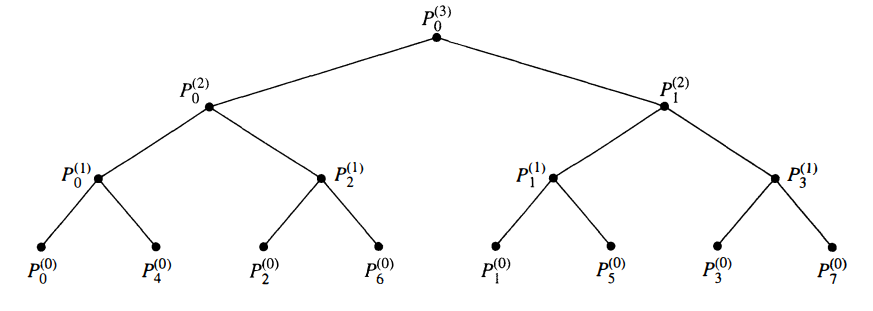
\includegraphics[scale=0.7]{../assets/tree.png}
    \end{center}
\end{mdframed}

\subsubsection{The Idea}
Each $P_{k}^{(n)}$ can be represented by a set of coefficients, $C_{kj}^{(n)}$, for $0 \leq n \leq m$ and $0 \leq k \leq 2^{m - n} - 1$ and $0 \leq j \leq 2^n - 1$. More specifically, the polynomial can be written as 
\[P_{k}^{(n)}(x) = \sum_{j = 0}^{2^{n} - 1} C_{kj}^{(n)} E_{j}(x) = \sum_{j = 0}^{2^{n} - 1} C_{kj}^{(m)} e^{ijx}.\]
Note that 
\[C_{kj}^{(n + 1)} = \frac{1}{2}\left(C_{kj}^{(n)} + e^{\frac{-ij\pi}{2^{n}}} C_{k + 2^{m - n - 1, j}}^{(m)}\right)\]
and 
\[C_{k, j + 2^{n}}^{(n + 1)} = \frac{1}{2}\left(C_{kj}^{(n)} - e^{\frac{-ij\pi}{2^{n}}} C_{k + 2^{m - n - 1, j}}^{(m)}\right)\]
So, for a fixed $n$ where $0 \leq k \leq 2^{m - n} - 1$ and $0 \leq j \leq 2^{n} - 1$, we have a matrix with $2^{m - n}$ rows and $2^n$ columns. Together, there's $2^{m - n} 2^n = 2^m = N$ entries. Instead, we'd like to map each matrix row to some elements in an array, something like 
\begin{center}
    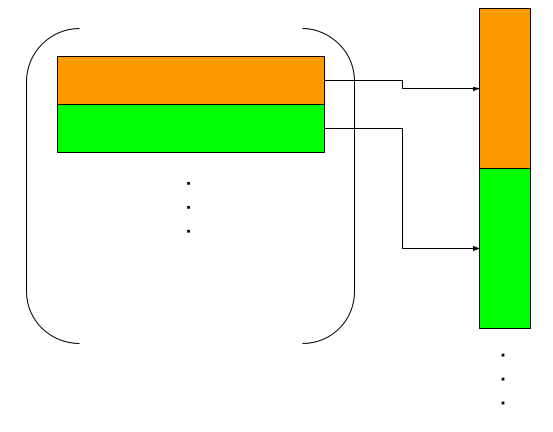
\includegraphics[scale=0.5]{../assets/matrix_to_arr.png}
\end{center}
The long array has $N$ elements in total. To get each element in this array, we can write 
\[C(2^{n}k + j) = C_{kj}^{(n)} \qquad 0 \leq k \leq 2^{m - n} = 1, 0 \leq j \leq 2^{n} - 1\]
\[D(2^{n + 1} k + j) = C_{kj}^{(n + 1)} \qquad 0 \leq k \leq 2^{m - n - 1} - 1, 0 \leq j \leq 2^{n + 1} - 1.\]
Next, we want to precompute $Z(j)$; that is, 
\[Z(j) = e^{-\frac{2\pi i j}{N}}\]
and write 
\[Z(j2^{m - n - 1}) = e^{-\frac{ij\pi}{2^n}}.\]

\subsection{The Algorithm}
With the ideas in mind, we can write the algorithm below. Note that this has inputs $m$ and $f(x)$. 
\begin{algorithm}[H]
    \caption{Fast Fourier Transform}
    \begin{algorithmic}[1]
        \Function{FFT}{$m, f$}
            \State $N \gets 2^m$
            \State $w \gets e^{-\frac{2\pi i}{N}}$
            \For{$k \gets 0$ to $N - 1$}
                \State $Z(k) \gets w^k$
                \State $C(k) \gets f\left(\frac{2\pi k}{N}\right)$
            \EndFor 

            \For{$n \gets 0$ to $m - 1$}
                \For{$k \gets 0$ to $2^{m - n - 1} = 1$}
                    \For{$j \gets 0$ to $2^n - 1$}
                        \State $u \gets C(2^n k + j)$
                        \State $v \gets Z(j2^{m - n - 1}) C(2^n k + 2^{m - 1} + j)$
                        \State $D(2^{n + 1} k + j) \gets \frac{u + v}{2}$
                        \State $D(2^{n + 1} k + j + 2^{n}) \gets \frac{u - v}{2}$
                    \EndFor 
                \EndFor 
                \For{$j \gets 0$ to $N - 1$}
                    \State $C(j) \gets D(j)$
                \EndFor 
            \EndFor 
            \State \textbf{return} $C$
        \EndFunction
    \end{algorithmic}
\end{algorithm}
The elements in $C$ can then be used in the interpolating formula (\ref{lec20px}).


\end{document}